\section{Linearity of the Radon transform}
It can be shown that the Radon transform is a linear transformation. By using the definition of \autoref{linearity} we can show:
\begin{align}
	\mathbf{R}\{\alpha f(x,y) + \beta g(x',y')\} &= \int_L \left(\alpha f(x,y) + \beta g(x',y')\right) dl\\
	&= \int_L \alpha f(x,y) dl + \int_L \beta g(x',y') dl \label{sumRule}\\
	&= \alpha \int_L f(x,y) dl + \beta \int_L g(x',y') dl \label{constantRule}\\
	&= \alpha \mathbf{R}\{f(x,y)\} + \beta \mathbf{R}\{g(x',y')\}
\end{align}
Where the sum rule is used in \autoref{sumRule} and the constant rule is used in \autoref{constantRule}. This shows the Radon transform is linear, and means adding two functions together and then taking the Radon transform is the same as taking the Radon transform and then adding the results together. This comes down to the line integrals used to achieve the projections. As images are discrete we can not comply exactly to the mathematical definitions with line integrals. Instead we can use a Riemann sum to approximate the line integrals, that is we can take the sum of pixel intensities along a line to approximate the line integrals. If we then take \autoref{linearityExplained} as an example, we have two uniform circles. If we imagine one is defined by $f(x,y)$ and the other by $g(x',y')$, then adding $f(x,y)$ and $g(x',y')$ together gives us \autoref{linearityExplained}. We can now quite intuitively see that taking the sum of pixel intensities along the lines shown \autoref{linearityExplained}, i.e. summing over the lines in $f(x,y) + g(x',y')$, would be the same as summing over the lines in first $f(x,y)$, then $g(x',y')$ and then finally add the results together.
\begin{figure}
	\centering
	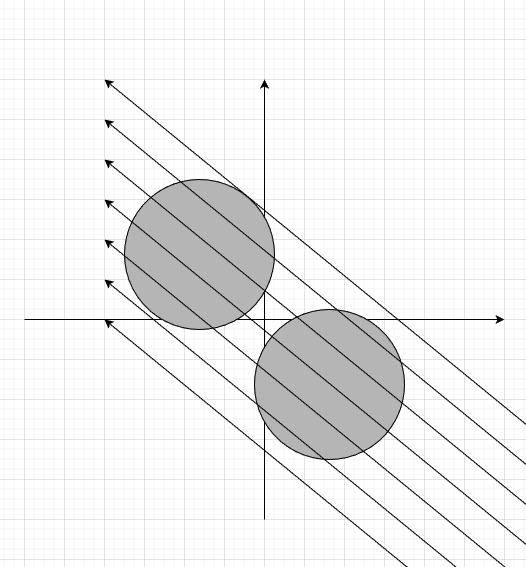
\includegraphics[width=\linewidth]{Materials/linearityExplained}
	\caption{Two uniform circles and the lines along which the line integrals are taken.}
	\label{linearityExplained}
\end{figure}